\documentclass[twoside, english]{hcmut-report}

%%% Optional packages
% \usepackage{}

%%% Configurations
\setstretch{1.2}
\setlength{\arraycolsep}{15pt}
\AtBeginDocument{\counterwithin{lstlisting}{section}}

%%% Custom commands
\newcommand{\inputfigure}[3][0.95]{
\begin{figure}[htbp]%
  \begin{center}%
    \includegraphics[width=#1\textwidth]{figures/#2}%
  \end{center}%
  \caption{#3}%
\end{figure}%
}

%%% Rename sections
% \AtBeginDocument{\renewcommand*{\contentsname}{Contents}}
% \AtBeginDocument{\renewcommand*{\refname}{References}}
% \AtBeginDocument{\renewcommand*{\bibname}{References}}

%%% MAIN DOCUMENT
\begin{document}
% \coverpage

\renewcommand{\thesection}{\Roman{section}}
\renewcommand{\thesubsubsection}{\thesubsection.\alph{subsubsection}}

\tableofcontents
% \listoffigures
% \listoftables
% \lstlistoflistings{}
\clearpage

\raggedbottom

\section{Muscle Force Density in a 3D Musculoskeletal Region}

\subsection{Problem Statement}
A biomechanics researcher analyzes a 3D musculoskeletal region where the
\textbf{muscle force density} is given by:
$$g(x,y,z) = 652.75x^{4}y^{8}z^{7}$$
over the region bounded by: $0 \le x \le 5$, $0 \le y \le 6$, $0 \le z \le 3$.
Compute the total muscle force distributed in the region.

\subsection{Detailed Solution}
\textit{ Sol. }

\begin{equation*}
	\begin{aligned}
		F & = \iiint_V g(x,y,z) \, dV                                                                                                  \\
		  & = \int_{0}^{3} \int_{0}^{6} \int_{0}^{5} 652.75x^{4}y^{8}z^{7} \, dx \, dy \, dz                                           \\
		  & = 652.75 \left( \int_{0}^{5} x^4 \, dx \right) \left( \int_{0}^{6} y^8 \, dy \right) \left( \int_{0}^{3} z^7 \, dz \right) \\
		  & = 652.75 \left[ \frac{x^5}{5} \right]_{0}^{5} \left[ \frac{y^9}{9} \right]_{0}^{6} \left[ \frac{z^8}{8} \right]_{0}^{3}    \\
		  & = 652.75 \left( 625 \right) \left( 1,119,744 \right) \left( 820.125 \right)                                                \\
		  & \approx \boxed{374,649,962,215,039.5000}
	\end{aligned}
\end{equation*}

\subsection{Matlab Implementation}
\begin{figure}[htbp]
	\begin{center}
		\includegraphics[width=0.95\textwidth]{figures/result01.png}
	\end{center}
	\caption{Student 04 - Matlab Screenshot}
	\label{stu4_ques1}
\end{figure}

\section{Force Distribution in a Spherical Joint Model}

\subsection{Problem Statement}
A biomechanics team models a spherical joint system with radius \textbf{7.5 units}, where the \textbf{joint force density} at a point $(x, y, z)$ is described by:
$$I(x,y,z) = 600.17x^{2} + 600.17y^{2} + 600.17z^{2}$$
Compute the total joint force in the system using \textbf{spherical coordinates}.

\subsection{Detailed Solution}
\textit{ Sol. }
\begin{equation*}
	\begin{aligned}
		              & \begin{cases}
			                I(\rho, \theta, \phi) & = 600.17(x^{2} + y^{2} + z^{2} ) = 600.17\rho^2 \\
			                dV                    & = \rho^2 \sin\phi \, d\rho \, d\phi \, d\theta
		                \end{cases}                                                                       \\[1em]
		\Rightarrow F & = \int_{0}^{2\pi} \int_{0}^{\pi} \int_{0}^{7.5} (600.17\rho^2)(\rho^2 \sin\phi) \, d\rho \, d\phi \, d\theta                                  \\
		              & = 600.17 \left( \int_{0}^{7.5} \rho^4 \, d\rho \right) \left( \int_{0}^{\pi} \sin\phi \, d\phi \right) \left( \int_{0}^{2\pi} d\theta \right) \\
		              & = 600.17 \Big[ \frac{\rho^5}{5} \Big]_{0}^{7.5} \Big[ -\cos\phi \Big]_{0}^{\pi} \Big[ \theta \Big]_{0}^{2\pi}                                 \\
		              & = 600.17 \left( \frac{151875}{32} \right) \left( 2 \right) \left( 2\pi \right)                                                                \\
		              & \approx \boxed{35,794,842.8185}
	\end{aligned}
	\label{eq:stu4q2}
\end{equation*}

\subsection{Matlab Implementation}
\begin{figure}[H]
	\begin{center}
		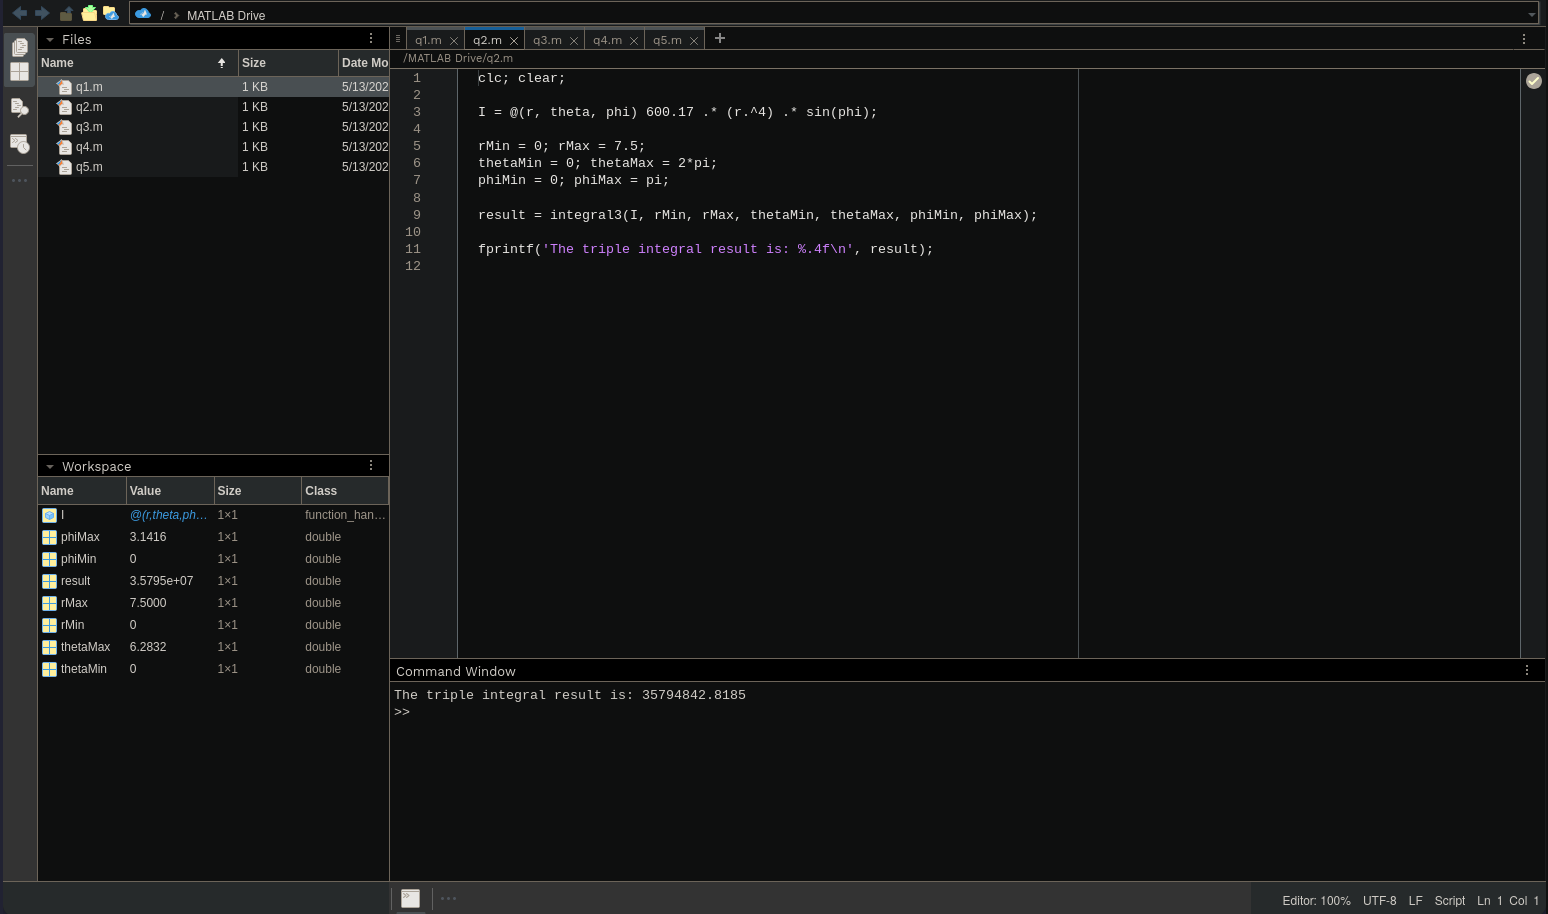
\includegraphics[width=0.95\textwidth]{figures/stu4q2.png}
	\end{center}
	\caption{Student 04 - Matlab Screenshot}
	\label{fig:stu4q2}
\end{figure}

\subsection{Conclusion}
By converting to spherical coordinates, the total joint force (Equation \ref{eq:stu4q2}) \textbf{does} match the MATLAB output (Figure \ref{fig:stu4q2}).

\subsubsection*{Problem Statement Question 3}
A cylindrical limb segment in a musculoskeletal model has a radius of \textbf{5.5 units} and a height of \textbf{9.5 units}. The \textbf{tendon stress density} at a point $(x,y,z)$ within the segment is defined by:
\[ P(x, y, z) = 354.62x^2 + 354.62y^2 \]
Compute the total tendon stress in the segment using \textbf{cylindrical coordinates}.

\subsubsection*{Solution}
The total tendon stress $S$ is defined as the triple integral of the density function $P(x, y, z)$ over the cylindrical region:
\[ S = \iiint_V P(x, y, z) \, dV \]

Converting the density function into cylindrical coordinates ($x^2 + y^2 = r^2$):
\[ P(r, \theta, z) = 354.62r^2 \]

The volume element in cylindrical coordinates is $dV = r \, dr \, d\theta \, dz$. The limits of integration for the cylinder are:
\[ 0 \le r \le 5.5, \quad 0 \le \theta \le 2\pi, \quad 0 \le z \le 9.5 \]

Applying the iterated integration process step-by-step:
\[ S = \int_{0}^{9.5} \int_{0}^{2\pi} \int_{0}^{5.5} 354.62r^3 \, dr \, d\theta \, dz \]

\vspace{1cm}
\noindent\textbf{Step 1: Integrate with respect to $r$.}

\[ \int_{0}^{5.5} 354.62r^3 \, dr = 354.62 \left[ \frac{r^4}{4} \right]_{0}^{5.5} \]
\[ = 354.62 \left( \frac{14641}{64} \right) = 81124.8759 \]
\[ \Rightarrow S = \int_{0}^{9.5} \int_{0}^{2\pi} 81124.8759 \, d\theta \, dz \]

\vspace{1cm}
\noindent\textbf{Step 2: Integrate with respect to $\theta$.}

\[ \int_{0}^{2\pi} 81124.8759 \, d\theta = 81124.8759 \Big[\theta\Big]_{0}^{2\pi} = 162249.7518\pi \]
The integral expression simplifies to:
\[ S = \int_{0}^{9.5} 162249.7518\pi \, dz \]

\vspace{1cm}
\noindent\textbf{Step 3: Integrate with respect to $z$.}

\[ \int_{0}^{9.5} 162249.7518\pi \, dz = 162249.7518\pi [z]_{0}^{9.5} = 162249.7518\pi (9.5) \]

\vspace{1cm}
\noindent\textbf{Step 4: Simplify the result.}

\[ S = 1540798.1171\pi \approx \boxed{4,842,364.3742} \]

Thus, the total tendon stress distributed in the segment is exactly $\mathbf{4,842,364.3742}$.

\subsubsection*{MATLAB Verification \& Conclusion}
\textbf{MATLAB Code:}
\begin{mdframed}[backgroundcolor=gray!10]
	\inputminted{matlab}{codes/q3s4.m}
\end{mdframed}

\vspace{1cm}
\noindent\textbf{MATLAB Screenshot:}
\begin{figure}[H]
	\begin{center}
		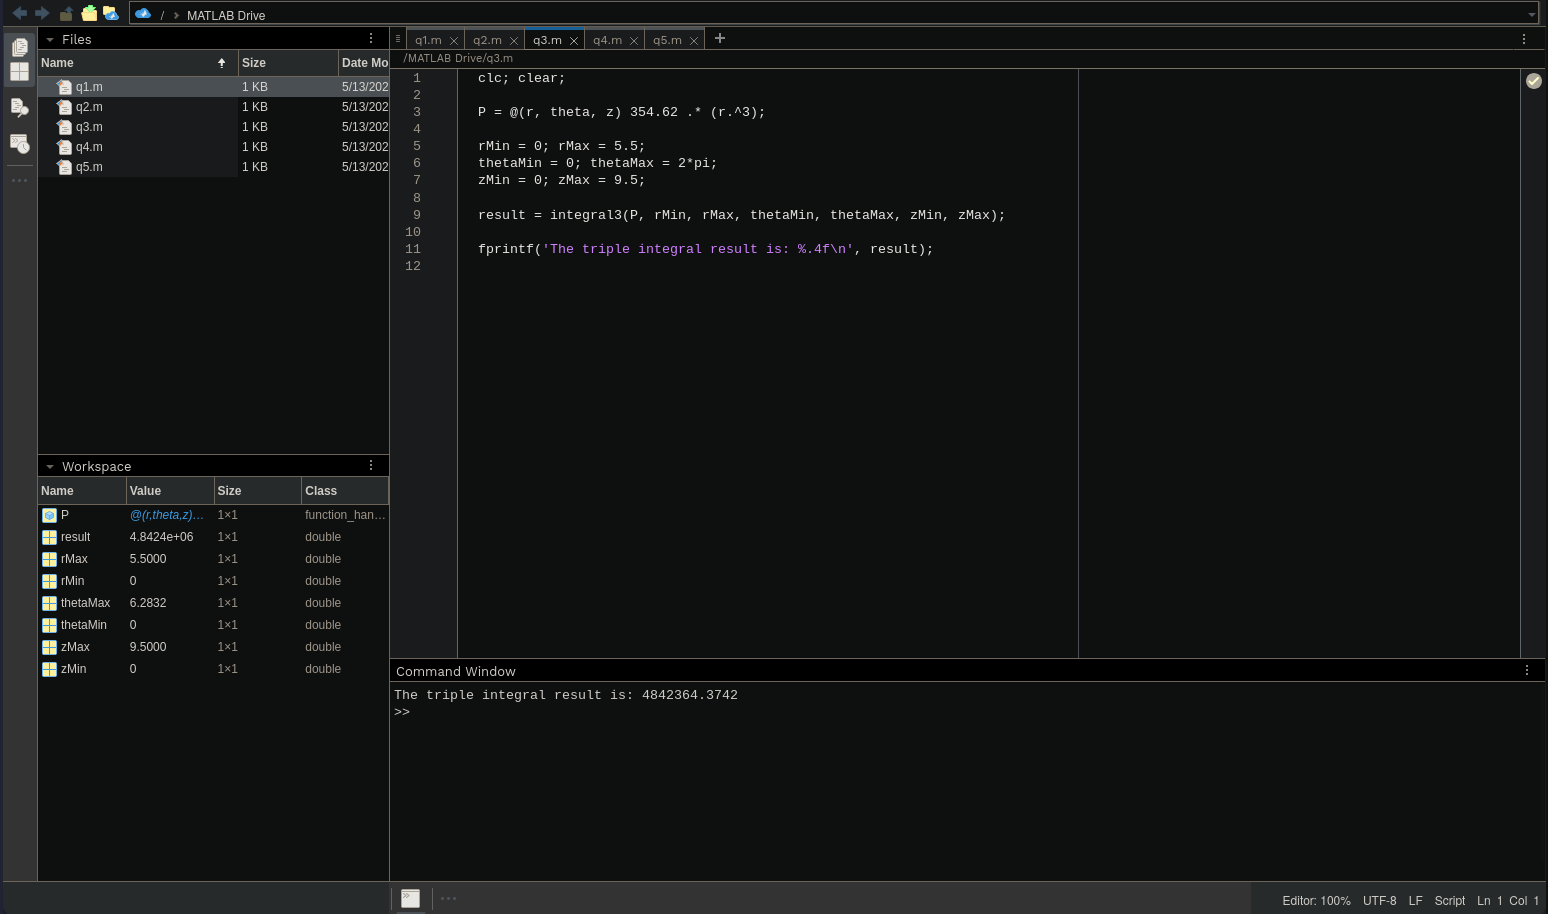
\includegraphics[width=0.95\textwidth]{figures/stu4q3.png}
	\end{center}
\end{figure}

\vspace{1cm}
\noindent\textbf{Conclusion:}

The total tendon stress calculated by using cylindrical coordinates gives the \textbf{same} result as the MATLAB script.

\section{Musculoskeletal Force Output}

\subsection{Problem Statement}
In a multivariable musculoskeletal model, the \textbf{force output density function} for a limb system is:
$$P(x, y, z) = 901.17xyz$$
where $x, y, z$ represent normalized inputs for muscle contraction, joint pressure, and bone displacement. A transformation to new coordinates is defined by:
$$x=\frac{u+3v+w}{7}, \quad y=\frac{u-v+w}{7}, \quad z=\frac{u-v-3w}{7}$$
Compute the \textbf{total musculoskeletal force output} over the region:
$0 \le u \le 3$, $-1 \le v \le 6$, $-1 \le w \le 4$, using the \textbf{Jacobian transform}.

\subsection{Detailed Solution}
\textit{ Sol. }
\begin{equation*}
	\begin{aligned}
		J & = \frac{\partial(x,y,z)}{\partial(u,v,w)} = \begin{vmatrix} 1/7 & 3/7 & 1/7 \\ 1/7 & -1/7 & 1/7 \\ 1/7 & -1/7 & -3/7 \end{vmatrix} \\
		  & = \left(\frac{1}{7}\right)^3 \begin{vmatrix} 1 & 3 & 1 \\ 1 & -1 & 1 \\ 1 & -1 & -3 \end{vmatrix}                                  \\
		  & = \frac{1}{343} \Big[ 1((-1)(-3) - (1)(-1)) - 3((1)(-3) - (1)(1)) + 1((1)(-1) - (-1)(1)) \Big]                                     \\
		  & = \frac{1}{343} \Big[ 1(3 + 1) - 3(-3 - 1) + 1(-1 + 1) \Big]                                                                       \\
		  & = \frac{16}{343}
	\end{aligned}
\end{equation*}

\begin{equation*}
	\Rightarrow dV = |J| \, du \, dv \, dw = \frac{16}{343} \, du \, dv \, dw
\end{equation*}

\begin{equation*}
	\begin{aligned}
		F & = \int_{-1}^{4} \int_{-1}^{6} \int_{0}^{3} 901.17 \left( \frac{u+3v+w}{7} \right) \left( \frac{u-v+w}{7} \right)           \\
		  & \qquad\qquad \times \left( \frac{u-v-3w}{7} \right) \frac{16}{343} \, du \, dv \, dw                                       \\
		  & \text{Let } A = u - v + w                                                                                                  \\
		F & = \frac{901.17 \times 16}{7^3 \times 343} \int_{-1}^{4} \int_{-1}^{6} \int_{0}^{3} A(A+4v)(A-4w) \, du \, dv \, dw         \\
		  & = 0.122557 \int_{-1}^{4} \int_{-1}^{6} \int_{0}^{3} \left( A^3 + 4(v-w)A^2 - 16vwA \right) \, du \, dv \, dw               \\
		  & = 0.122557 \int_{-1}^{4} \int_{-1}^{6} \left[ \frac{A^4}{4} + \frac{4(v-w)A^3}{3} - 8vwA^2 \right]_{u=0}^{u=3} \, dv \, dw \\
		  & = 0.122557 \int_{-1}^{4} \int_{-1}^{6} \Big( 9v^3 + (21w - 22.5)v^2                                                        \\
		  & \qquad\qquad - (21w^2 + 27w - 9)v - (9w^3 + 22.5w^2 + 9w - 20.25) \Big) \, dv \, dw                                        \\
		  & = 0.122557 \int_{-1}^{4} \left( -63w^3 - 525w^2 + 983.5w + 1585.5 \right) \, dw                                            \\
		  & = 0.122557 \left[ \frac{-63w^4}{4} - \frac{525w^3}{3} + \frac{983.5w^2}{2} + 1585.5w \right]_{-1}^{4}                      \\
		  & = 0.122557 (-87.5)                                                                                                         \\
		  & \approx \boxed{-10.7237}
	\end{aligned}
\end{equation*}

\subsection{Matlab Implementation}
\begin{figure}[htbp]
	\begin{center}
		\includegraphics[width=0.95\textwidth]{figures/result04.png}
	\end{center}
	\caption{Student 04 - Matlab Screenshot}
	\label{stu4_ques4}
\end{figure}

\section{Force Cost Evaluation in a Tetrahedral Musculoskeletal System}

\subsection{Problem Statement}
The following triple integral represents the \textbf{force cost function} in a bounded musculoskeletal system with quadratic variation along the vertical axis:
$$\iiint_{E}(480.92x+592.03y+z^{2})dV$$
where $E$ is the solid tetrahedron bounded by: $x=0.1$, $y=0.3$, $z=0.4$, $x+y+z=5$. Evaluate the \textbf{total force cost} within the system.

\subsection{Detailed Solution}
\textit{ Sol. }
\begin{itemize}
	\item \textbf{Inner bounds ($z$):} $ x + y + z = 5 \Rightarrow z \in{[ 0.4,\ 5 - x - y ]} $
	\item \textbf{Middle bounds ($y$):} $ z_{\text{min}} = 0.4 \Rightarrow y \in{[ 0.3,\ 5 - 0.4 - x]} \iff y \in{[ 0.3,\ 4.6 - x]}  $
	\item \textbf{Outer bounds ($x$):} $ y_{\text{min}} = 0.3,\ z_{\text{min}} = 0.4 \Rightarrow x \in{[ 0.3,\ 5 - 0.3 - 0.4]} \iff x \in{[ 0.3,\ 4.3]} $
\end{itemize}

\begin{equation*}
	\begin{aligned}
		C & = \iiint_{E}(480.92x+592.03y+z^{2}) \, dV                                                                                            \\
		  & = \int_{0.1}^{4.3} \int_{0.3}^{4.6-x} \int_{0.4}^{5-x-y} (480.92x + 592.03y + z^2) \, dz \, dy \, dx                                 \\
		  & = \int_{0.1}^{4.3} \int_{0.3}^{4.6-x} \left[ (480.92x + 592.03y)z + \frac{z^3}{3} \right]_{0.4}^{5-x-y} \, dy \, dx                  \\
		  & = \int_{0.1}^{4.3} \int_{0.3}^{4.6-x} \Bigg( (480.92x + 592.03y)(4.6-x-y)                                                            \\
		  & \qquad\qquad + \frac{(5-x-y)^3}{3} - \frac{0.064}{3} \Bigg) \, dy \, dx                                                              \\
		  & = \int_{0.1}^{4.3} \Bigg[ 480.92x \left((4.6-x)y - \frac{y^2}{2}\right) + 592.03 \left( \frac{(4.6-x)y^2}{2} - \frac{y^3}{3} \right) \\
		  & \qquad\qquad - \frac{(5-x-y)^4}{12} - \frac{0.064y}{3} \Bigg]_{y=0.3}^{y=4.6-x} \, dx                                                \\
		  & = \int_{0.1}^{4.3} \Bigg( 240.46x(4.6-x)^2 + \frac{592.03}{6}(4.6-x)^3 - \frac{0.064(4.6-x)}{3} - \frac{0.4^4}{12}                   \\
		  & \qquad\qquad - 480.92x(1.335 - 0.3x) - 592.03(0.045(4.6-x) - 0.009) + \frac{(4.7-x)^4}{12} + 0.0064 \Bigg) \, dx                     \\
		  & = \Bigg[ 240.46\left(\frac{x^4}{4} - \frac{9.2x^3}{3} + \frac{21.16x^2}{2}\right) - \frac{592.03(4.6-x)^4}{24}                       \\
		  & \qquad\qquad + \frac{0.04(4.6-x)^2}{6} - \frac{0.0256x}{12} - 480.92\left(\frac{1.335x^2}{2} - \frac{0.3x^3}{3}\right)               \\
		  & \qquad\qquad + \frac{26.64135(4.6-x)^2}{2} + 5.32827x - \frac{(4.7-x)^5}{60} + 0.0064x \Bigg]_{0.1}^{4.3}                            \\
		  & \approx \boxed{16,732.3117}
	\end{aligned}
	\label{eq:stu4q5}
\end{equation*}

\subsection{Matlab Implementation}
\begin{figure}[H]
	\begin{center}
		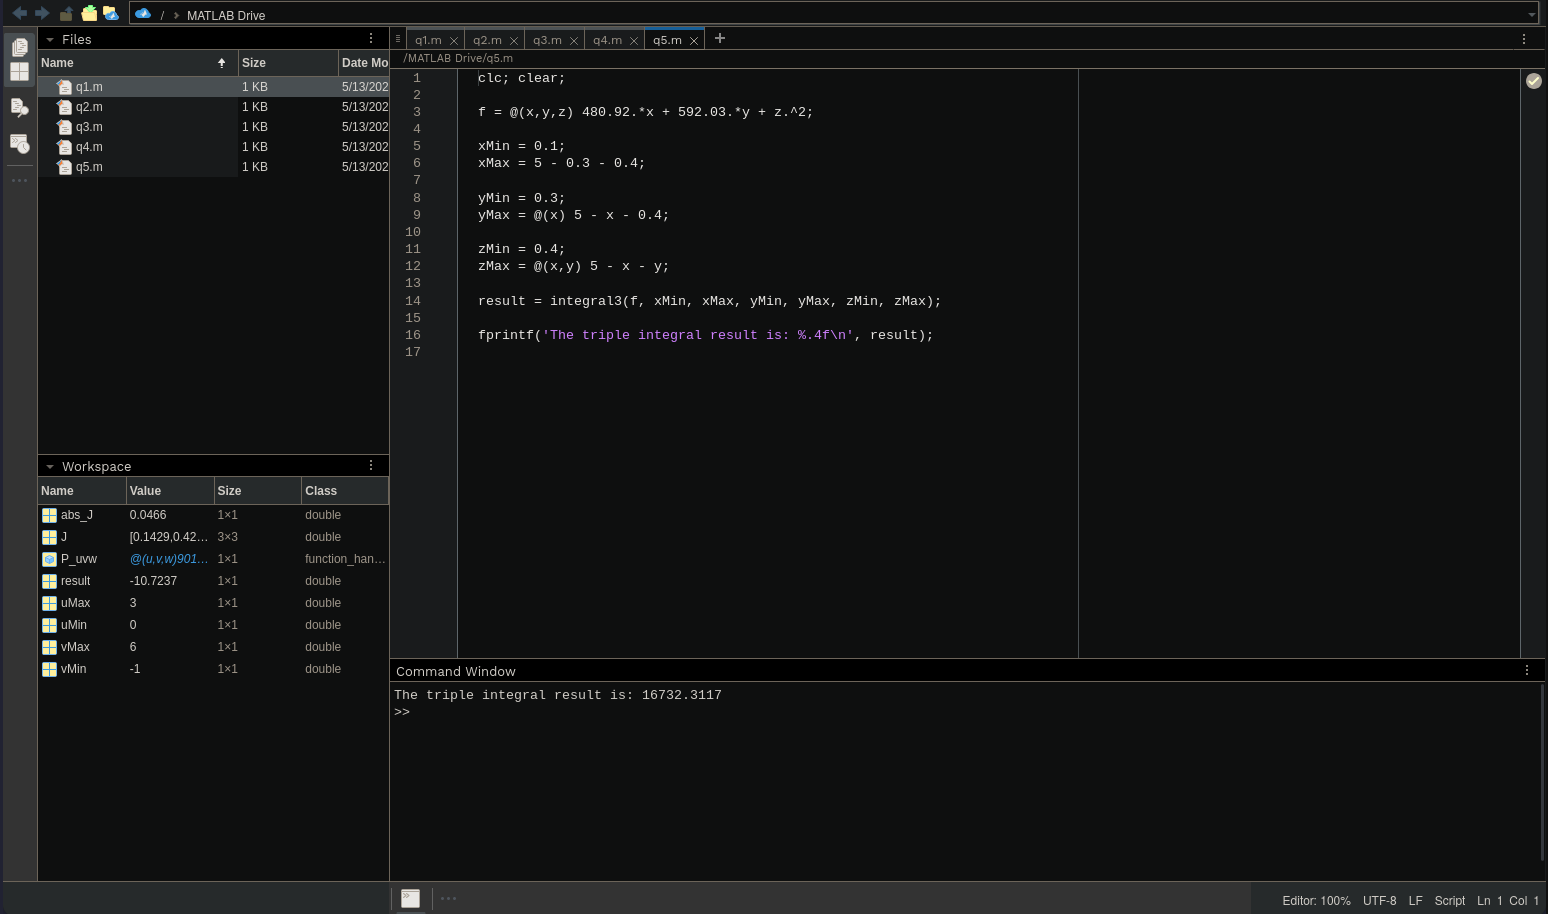
\includegraphics[width=0.95\textwidth]{figures/stu4q5.png}
	\end{center}
	\caption{Student 04 - Matlab Screenshot}
	\label{fig:stu4q5}
\end{figure}

\subsection{Conclusion}
The integration over the tetrahedral region (Equation \ref{eq:stu4q5}) results in the \textbf{same} value as the MATLAB script (Figure \ref{fig:stu4q5}).


% \begin{noindent}
% \begingroup
%   \raggedright
%     \bibliographystyle{apacite}
%     \bibliography{refs/refs.bib}
%   \nocite{*}
% \endgroup
% \end{noindent}

% \clearpage
% \appendix

\end{document}
